\documentclass[tikz,border=2pt]{standalone}
\usepackage{amsmath,amssymb}
\usepackage{tikz}

\begin{document}
% Two joint pmfs on {0,1}^2 drawn as discs with area proportional to the mass: a general table
% and the fully dependent pair X = Y ~ Bern(1/2).
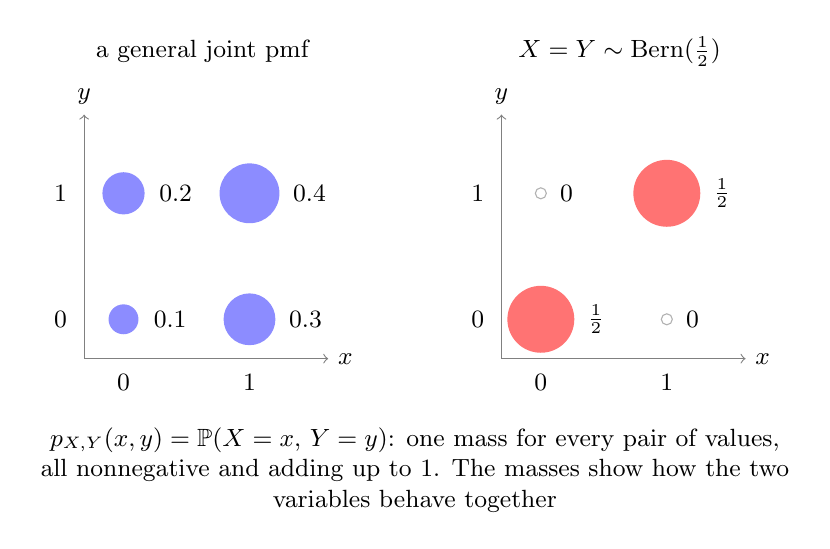
\begin{tikzpicture}[every node/.style={font=\small}]
	\begin{scope}
		\draw[->, gray] (-0.5,-0.5) -- (2.6,-0.5) node[right, black] {$x$};
		\draw[->, gray] (-0.5,-0.5) -- (-0.5,2.6) node[above, black] {$y$};
		\foreach \v/\p in {0/0, 1/1.6} {
			\node[font=\small] at (\p,-0.8) {$\v$};
			\node[font=\small] at (-0.8,\p) {$\v$};
		}
		\fill[blue!45] (0,0) circle (0.19);
		\fill[blue!45] (0,1.6) circle (0.268);
		\fill[blue!45] (1.6,0) circle (0.329);
		\fill[blue!45] (1.6,1.6) circle (0.38);
		\node[font=\small, anchor=west] at (0.26,0) {$0.1$};
		\node[font=\small, anchor=west] at (0.33,1.6) {$0.2$};
		\node[font=\small, anchor=west] at (1.98,0) {$0.3$};
		\node[font=\small, anchor=west] at (2.03,1.6) {$0.4$};
		\node at (1.0,3.4) {a general joint pmf};
	\end{scope}
	\begin{scope}[xshift=5.3cm]
		\draw[->, gray] (-0.5,-0.5) -- (2.6,-0.5) node[right, black] {$x$};
		\draw[->, gray] (-0.5,-0.5) -- (-0.5,2.6) node[above, black] {$y$};
		\foreach \v/\p in {0/0, 1/1.6} {
			\node[font=\small] at (\p,-0.8) {$\v$};
			\node[font=\small] at (-0.8,\p) {$\v$};
		}
		\fill[red!55] (0,0) circle (0.425);
		\fill[red!55] (1.6,1.6) circle (0.425);
		\draw[gray!60] (0,1.6) circle (0.07);
		\draw[gray!60] (1.6,0) circle (0.07);
		\node[font=\small, anchor=west] at (0.47,0) {$\tfrac12$};
		\node[font=\small, anchor=west] at (2.07,1.6) {$\tfrac12$};
		\node[font=\small, anchor=west] at (0.12,1.6) {$0$};
		\node[font=\small, anchor=west] at (1.72,0) {$0$};
		\node at (1.0,3.4) {$X=Y\sim\operatorname{Bern}(\tfrac12)$};
	\end{scope}
	\node[anchor=north, align=flush center, text width=9.6cm] at (3.7,-1.25) {$p_{X,Y}(x,y)=\mathbb{P}(X=x,\,Y=y)$: one mass for every pair of values, all nonnegative and adding up to $1$. The masses show how the two variables behave together};
\end{tikzpicture}
\end{document}
